% Figure 1: Two-ended asymptotic geometry and energy-dependent channel
% structure of the massive Kerr-Dirac equation.
% Authors: Dr. Davide Batic and Dr. Denys Dutykh
%          (Mathematics Department, Khalifa University of Science and
%           Technology, Abu Dhabi, UAE)
\documentclass[tikz,border=6pt]{standalone}
% ============================================================================
% Shared TikZ style for the figures of the Kerr–Dirac two-channel scattering
% manuscript (compiled standalone into ../latex/figures/).
% Authors: Dr. Davide Batic and Dr. Denys Dutykh
%          (Mathematics Department, Khalifa University of Science and
%           Technology, Abu Dhabi, UAE)
%
% Visual language (used consistently across all figures):
%   * horizon channel      : navy  (chH)
%   * spatial-infinity     : teal  (chI)
%   * accents / emphasis   : gold  (acc)
%   * future/out data      : solid arrows
%   * past/in data         : dashed arrows
%   * proved here          : solid box border
%   * imported input       : light-gray filled box
%   * conditional          : dashed box border
% ============================================================================
\usepackage{amsmath,amssymb}
\usetikzlibrary{arrows.meta,positioning,decorations.pathmorphing,calc,matrix}

\definecolor{chH}{HTML}{142D6E}   % horizon channel (navy)
\definecolor{chI}{HTML}{0E6E6E}   % spatial-infinity channel (teal)
\definecolor{acc}{HTML}{9A7A2E}   % gold accent
\definecolor{warm}{HTML}{9C5310}  % sienna (warnings/exclusions)
\definecolor{ltg}{HTML}{F2F2F2}   % light gray fill (imported)

\tikzset{
  outarr/.style={-{Stealth[length=2.6mm]}, line width=0.9pt},
  inarr/.style={-{Stealth[length=2.6mm]}, line width=0.9pt, dashed},
  axis/.style={-{Stealth[length=2.2mm]}, line width=0.6pt, gray!70!black},
  wavyH/.style={chH, decorate, decoration={snake, amplitude=0.45mm, segment length=2.6mm}},
  wavyI/.style={chI, decorate, decoration={snake, amplitude=0.45mm, segment length=2.6mm}},
  proved/.style={draw, line width=0.7pt, rounded corners=2pt, inner sep=4pt},
  imported/.style={draw=gray!60, fill=ltg, line width=0.5pt, rounded corners=2pt, inner sep=4pt},
  conditional/.style={draw, dashed, line width=0.7pt, rounded corners=2pt, inner sep=4pt},
  lab/.style={font=\small},
  slab/.style={font=\footnotesize},
  tlab/.style={font=\scriptsize},
}

\begin{document}
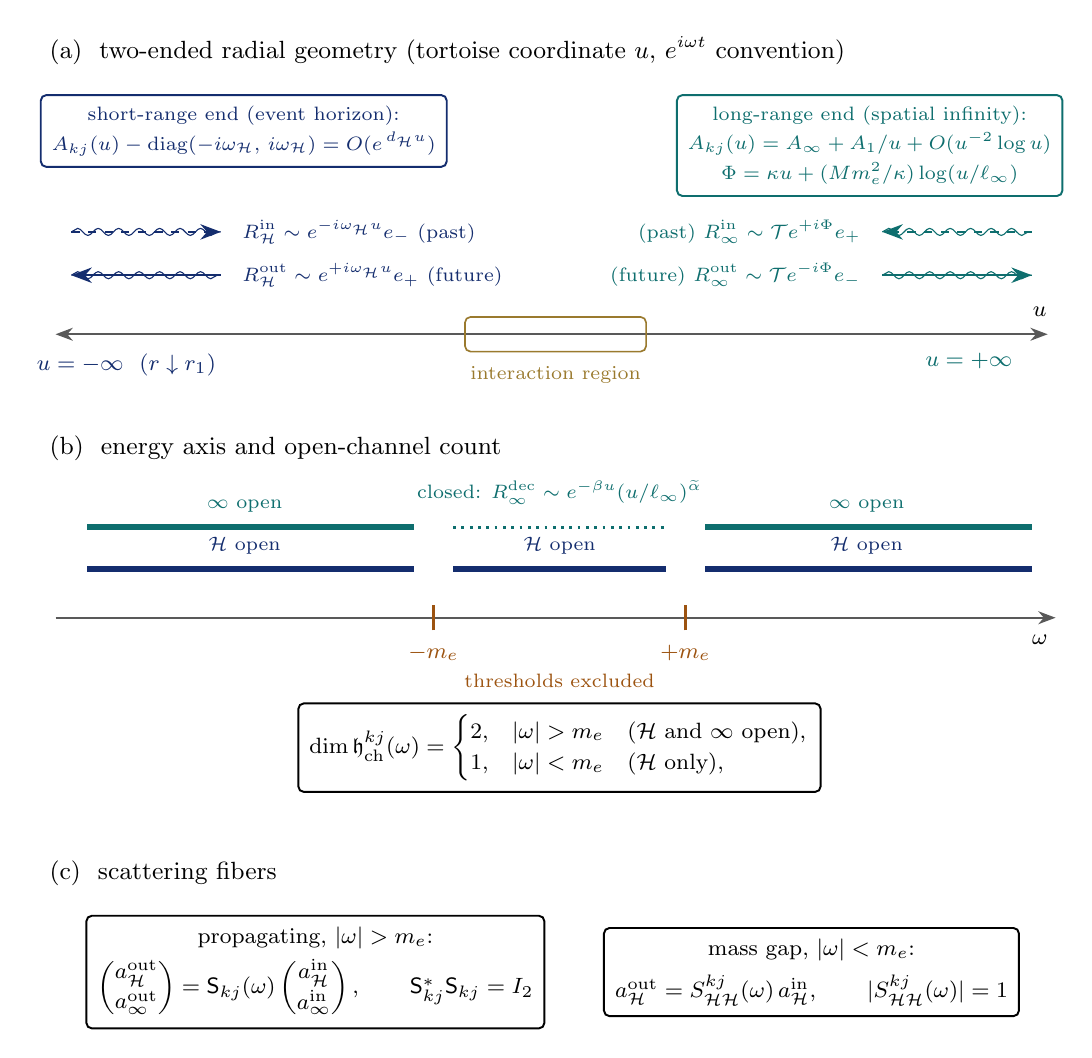
\begin{tikzpicture}[x=1cm,y=1cm]

% ===================== panel (a): radial scattering geometry ================
\begin{scope}[shift={(0,0)}]
  \node[lab, anchor=west] at (-0.4,3.6) {(a)\ \ two-ended radial geometry (tortoise coordinate $u$, $e^{i\omega t}$ convention)};
  % info boxes
  \node[proved, chH, tlab, align=center, anchor=north west] at (-0.4,3.05)
    {\textcolor{chH}{short-range end (event horizon):}\\[0.5mm]
     $A_{kj}(u)-\mathrm{diag}(-i\omega_{\mathcal H},\,i\omega_{\mathcal H})=O(e^{\,d_{\mathcal H}u})$};
  \node[proved, chI, tlab, align=center, anchor=north east] at (12.6,3.05)
    {\textcolor{chI}{long-range end (spatial infinity):}\\[0.5mm]
     $A_{kj}(u)=A_\infty+A_1/u+O(u^{-2}\log u)$\\[0.5mm]
     $\Phi=\kappa u+(Mm_e^{2}/\kappa)\log(u/\ell_\infty)$};
  % mode lines with labels placed toward the centre
  \draw[wavyH] (0.0,1.30) -- (1.9,1.30);
  \draw[inarr, chH] (0.0,1.30) -- (1.9,1.30);
  \node[tlab, chH, anchor=west] at (2.05,1.30)
    {$R_{\mathcal H}^{\rm in}\sim e^{-i\omega_{\mathcal H}u}e_-$ (past)};
  \draw[wavyH] (0.0,0.75) -- (1.9,0.75);
  \draw[outarr, chH] (1.9,0.75) -- (0.0,0.75);
  \node[tlab, chH, anchor=west] at (2.05,0.75)
    {$R_{\mathcal H}^{\rm out}\sim e^{+i\omega_{\mathcal H}u}e_+$ (future)};
  \draw[wavyI] (10.3,1.30) -- (12.2,1.30);
  \draw[inarr, chI] (12.2,1.30) -- (10.3,1.30);
  \node[tlab, chI, anchor=east] at (10.15,1.30)
    {(past) $R_\infty^{\rm in}\sim \mathcal T e^{+i\Phi}e_+$};
  \draw[wavyI] (10.3,0.75) -- (12.2,0.75);
  \draw[outarr, chI] (10.3,0.75) -- (12.2,0.75);
  \node[tlab, chI, anchor=east] at (10.15,0.75)
    {(future) $R_\infty^{\rm out}\sim \mathcal T e^{-i\Phi}e_-$};
  % axis
  \draw[axis, {Stealth[length=2.2mm]}-{Stealth[length=2.2mm]}] (-0.2,0) -- (12.4,0);
  \node[slab, anchor=south] at (12.3,0.10) {$u$};
  \node[slab, chH, anchor=north] at (0.7,-0.12) {$u=-\infty$\ \ ($r\downarrow r_1$)};
  \node[slab, chI, anchor=north] at (11.4,-0.12) {$u=+\infty$};
  \draw[acc, line width=0.6pt, rounded corners=2pt] (5.0,-0.22) rectangle (7.3,0.22);
  \node[tlab, acc, anchor=north] at (6.15,-0.28) {interaction region};
\end{scope}

% ===================== panel (b): energy axis and channel count =============
\begin{scope}[shift={(0,-3.6)}]
  \node[lab, anchor=west] at (-0.4,2.15) {(b)\ \ energy axis and open-channel count};
  % channel lanes
  \draw[chI, line width=2.2pt] (0.2,1.15) -- (4.35,1.15);
  \draw[chI, line width=2.2pt] (8.05,1.15) -- (12.2,1.15);
  \node[tlab, chI, anchor=south] at (2.2,1.22) {$\infty$ open};
  \node[tlab, chI, anchor=south] at (10.1,1.22) {$\infty$ open};
  \draw[chI, line width=1.0pt, dotted] (4.85,1.15) -- (7.55,1.15);
  \node[tlab, chI, anchor=south] at (6.2,1.32)
    {closed: $R_\infty^{\rm dec}\sim e^{-\beta u}(u/\ell_\infty)^{\widetilde\alpha}$};
  \draw[chH, line width=2.2pt] (0.2,0.62) -- (4.35,0.62);
  \draw[chH, line width=2.2pt] (4.85,0.62) -- (7.55,0.62);
  \draw[chH, line width=2.2pt] (8.05,0.62) -- (12.2,0.62);
  \node[tlab, chH, anchor=south] at (2.2,0.68) {$\mathcal H$ open};
  \node[tlab, chH, anchor=south] at (6.2,0.68) {$\mathcal H$ open};
  \node[tlab, chH, anchor=south] at (10.1,0.68) {$\mathcal H$ open};
  % axis with thresholds
  \draw[axis] (-0.2,0) -- (12.5,0);
  \node[slab, anchor=north] at (12.3,-0.10) {$\omega$};
  \foreach \x/\l in {4.6/{-m_e}, 7.8/{+m_e}}{
    \draw[warm, line width=1.1pt] (\x,-0.16) -- (\x,0.16);
    \node[slab, warm, anchor=north] at (\x,-0.22) {$\l$};}
  \node[tlab, warm] at (6.2,-0.80) {thresholds excluded};
  % dimension formula
  \node[proved, slab, align=center] at (6.2,-1.65)
    {$\dim\mathfrak h^{kj}_{\rm ch}(\omega)=
      \begin{cases}2, & |\omega|>m_e\quad(\mathcal H\ \text{and}\ \infty\ \text{open}),\\
                   1, & |\omega|<m_e\quad(\mathcal H\ \text{only}),\end{cases}$};
\end{scope}

% ===================== panel (c): scattering fibers =========================
\begin{scope}[shift={(0,-8.1)}]
  \node[lab, anchor=west] at (-0.4,1.25) {(c)\ \ scattering fibers};
  \node[proved, slab, align=center] at (3.1,0)
    {propagating, $|\omega|>m_e$:\\[1mm]
     $\begin{pmatrix} a^{\rm out}_{\mathcal H}\\[0.5mm] a^{\rm out}_{\infty}\end{pmatrix}
      =\mathsf S_{kj}(\omega)
      \begin{pmatrix} a^{\rm in}_{\mathcal H}\\[0.5mm] a^{\rm in}_{\infty}\end{pmatrix},
      \qquad \mathsf S_{kj}^{*}\mathsf S_{kj}=I_2$};
  \node[proved, slab, align=center] at (9.4,0)
    {mass gap, $|\omega|<m_e$:\\[1.4mm]
     $a^{\rm out}_{\mathcal H}=S^{kj}_{\mathcal H\mathcal H}(\omega)\,a^{\rm in}_{\mathcal H},
      \qquad |S^{kj}_{\mathcal H\mathcal H}(\omega)|=1$};
\end{scope}

\end{tikzpicture}
\end{document}
